\documentclass{beamer}
\setbeamertemplate{navigation symbols}{}

\usepackage{tikz}
\graphicspath{{..//src//images//}}

\setbeamercolor{frametitle}{fg=black,bg=white}
\setbeamercolor{title}{fg=black,bg=yellow!85!orange}
\usetheme{AnnArbor}

\beamersetuncovermixins{\opaqueness<1>{25}}{\opaqueness<2->{15}}
\begin{document}
\title{Clustering Overview}
\author{FRI}
\date{\today} 

\begin{frame}
\titlepage
\end{frame}

\begin{frame}
\frametitle{What is clustering?}
    \begin{itemize}
    \item Partitioning into groups of similar objects
    \item Tens of algorithms
    \end{itemize}

\begin{center}
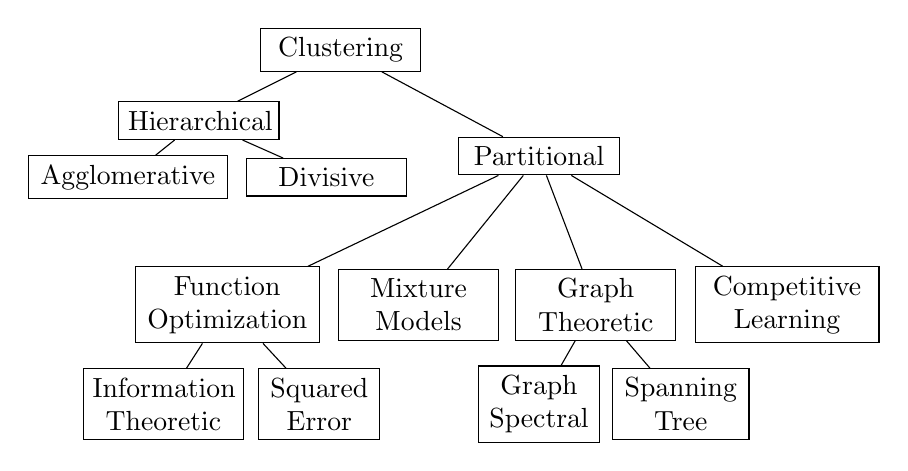
\begin{tikzpicture}[scale=0.9, text width=1.8cm, text centered]
    \tikzstyle{every node} = [rectangle,draw]

    \node (a) at (7, 5) {Clustering};
    \node (b) at (5, 4) {Hierarchical};
    \node (c) at (9.8, 3.5) {Partitional};

    \node (d) at (4, 3.2) [text width=2.3cm] {Agglomerative};
    \node (e) at (6.8, 3.2) {Divisive};

    \node (f) at (5.4, 1.4) [text width=2.1cm] {Function \\ Optimization};
    \node (g) at (8.1, 1.4) {Mixture \\ Models};
    \node (h) at (10.6, 1.4) {Graph \\ Theoretic};
    \node (i) at (13.3, 1.4) [text width=2.1cm] {Competitive \\ Learning};

    \node (j) at (4.5, 0.0) {Information \\ Theoretic};
    \node (k) at (6.7, 0.0) [text width=1.3cm] {Squared \\ Error};

    \node (l) at (9.8, 0.0) [text width=1.3cm] {Graph \\ Spectral};
    \node (m) at (11.8, 0.0) [text width=1.5cm] {Spanning \\ Tree};

    \draw [-] (a) -- (b);
    \draw [-] (a) -- (c);

    \draw [-] (b) -- (d);
    \draw [-] (b) -- (e);

    \draw [-] (c) -- (f);
    \draw [-] (c) -- (g);
    \draw [-] (c) -- (h);
    \draw [-] (c) -- (i);

    \draw [-] (f) -- (j);
    \draw [-] (f) -- (k);

    \draw [-] (h) -- (l);
    \draw [-] (h) -- (m);
\end{tikzpicture}
\end{center}

\end{frame}

\begin{frame}
\frametitle{k-means}
    \begin{itemize}
    \item Well-known and widely used
    \item Centroid-based, squared error minimization
    \item Fast but produces equi-sized clusters (Voronoi)
    \item Examples assigned to the closest cluster, centroids updated, repeat until convergence
    \item Improvements: k-means++ initialization
    \end{itemize}
\end{frame}

%\begin{frame}
%\frametitle{Applications of Clustering}
    %\begin{columns}[t]
        %\begin{column}[T]{9cm}
        %\begin{itemize}
        %\item YCbCr image compression
        %\item Reading digits from images (Google)
        %\end{itemize}

        %\vspace{10mm}
        %\hspace{7mm}
        %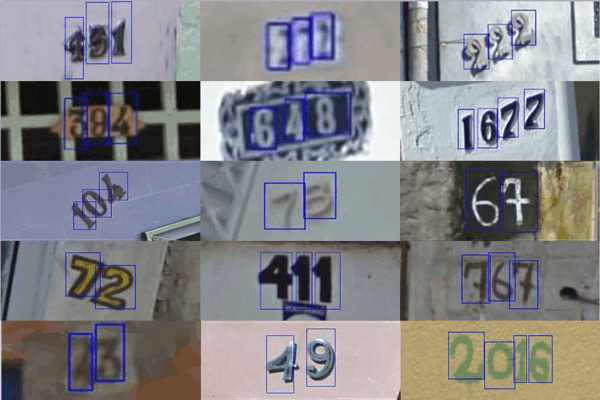
\includegraphics[height=4cm]{googlehousenumbers.jpg}

        %\end{column}

        %\begin{column}[T]{10cm}
        %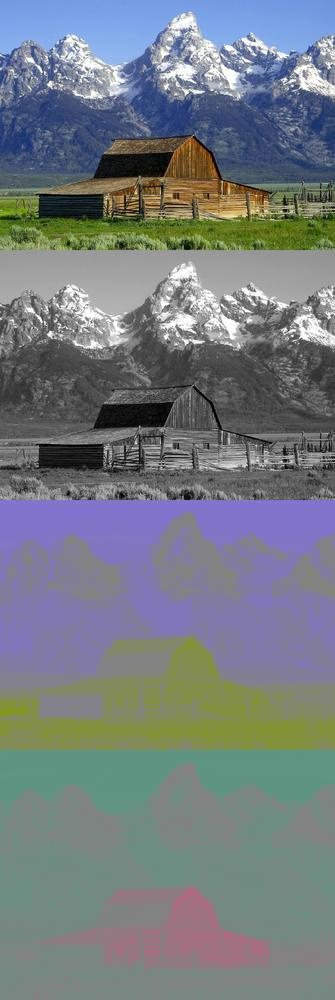
\includegraphics[height=7cm]{YCbCr-separation-small.jpg}
        %\end{column}
    %\end{columns}
%\end{frame} 

%\begin{frame}
%\frametitle{YCbCr image compression}
    %\begin{itemize}
    %\item Human eye more sensitive to brightness than color
    %\item Can reduce the bandwith of the chrominance channels
    %\item Chroma subsampling
    %\item NTSC, PAL, MPEG, JPEG
    %\item Color quantization
    %\end{itemize}
%\end{frame}

%\begin{frame}
%\frametitle{YCbCr image compression}
    %\begin{figure}[htb]
    %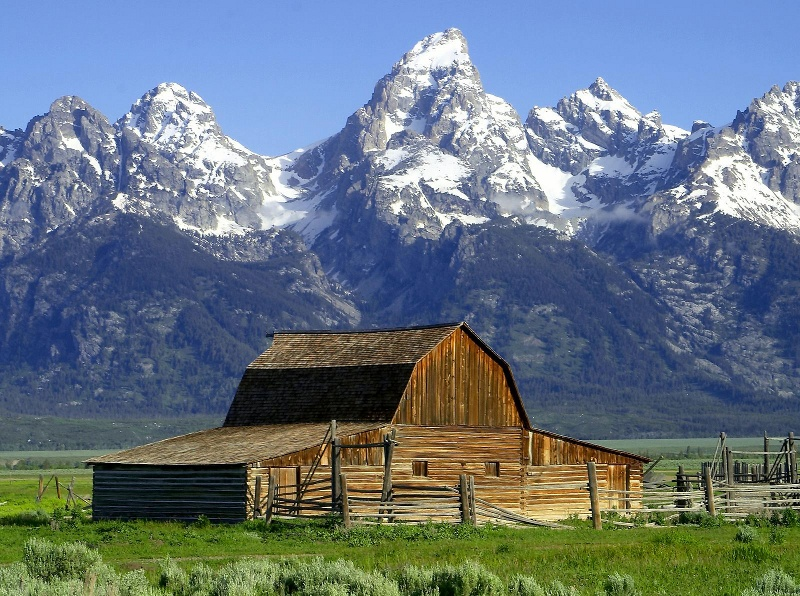
\includegraphics[scale=0.3]{YCbCr-normal.jpg}
    %\end{figure}
%\end{frame}

%\begin{frame}
%\frametitle{YCbCr image compression}
    %\begin{figure}[htb]
    %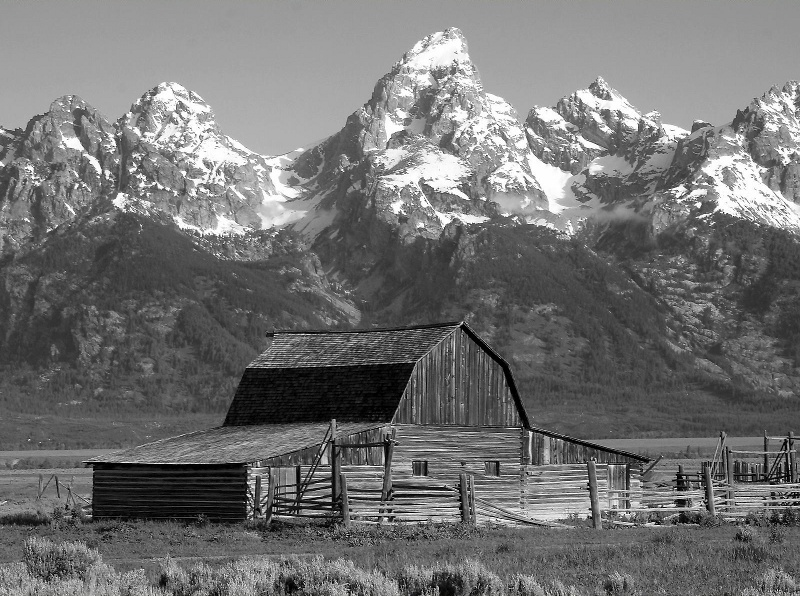
\includegraphics[scale=0.3]{YCbCr-bw.jpg}
    %\end{figure}
%\end{frame}

%\begin{frame}
%\frametitle{YCbCr image compression}
    %\begin{figure}[htb]
    %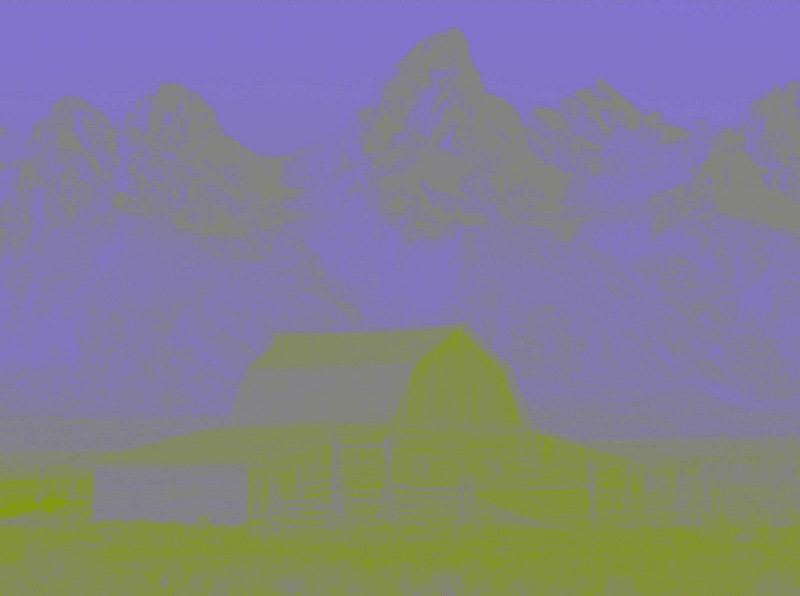
\includegraphics[scale=0.3]{YCbCr-cb.jpg}
    %\end{figure}
%\end{frame}

%\begin{frame}
%\frametitle{YCbCr image compression}
    %\begin{figure}[htb]
    %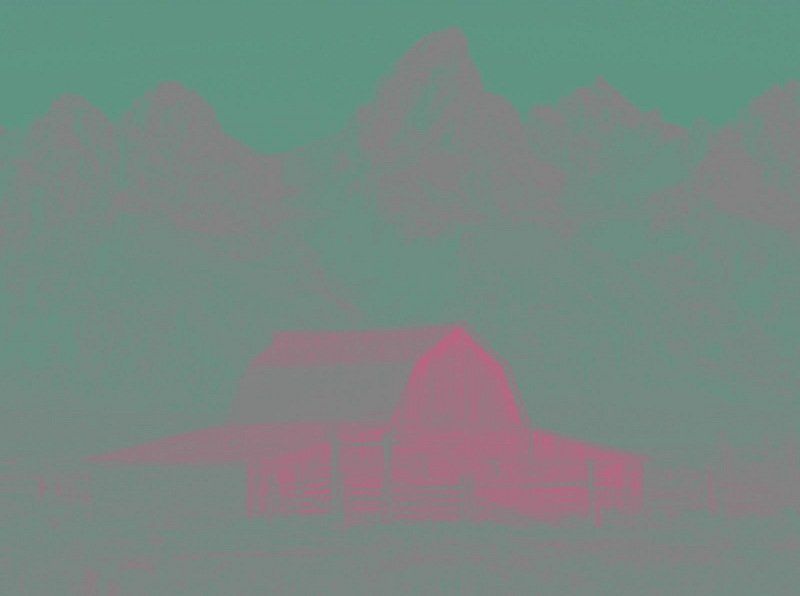
\includegraphics[scale=0.3]{YCbCr-cr.jpg}
    %\end{figure}
%\end{frame}

%\begin{frame}
%\frametitle{Podatki}
    %\begin{itemize}
        %\item Red-Blue
            %\begin{figure}[]
                %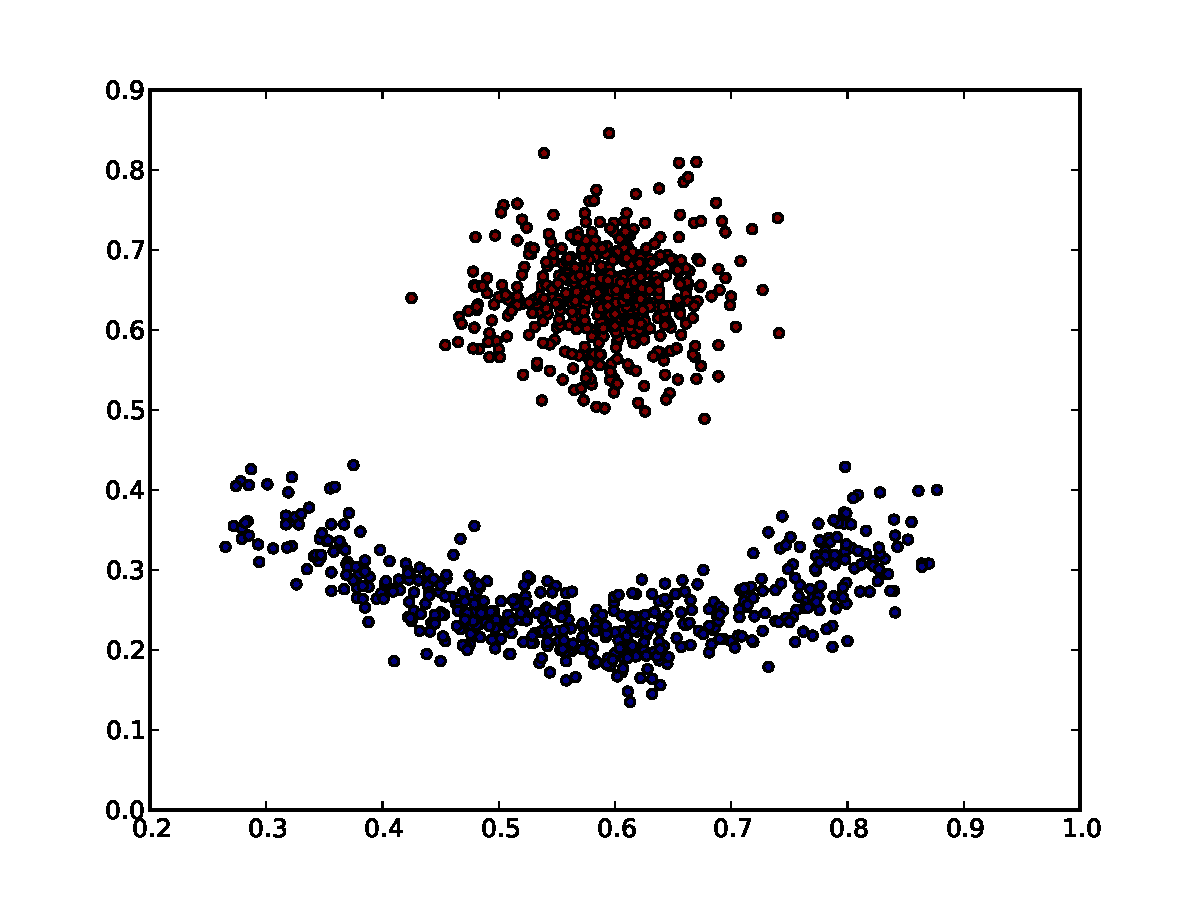
\includegraphics[scale=0.2]{red-blue-clusters.pdf}
            %\end{figure}
       %\item Nested-Circle
            %\begin{figure}[]
                %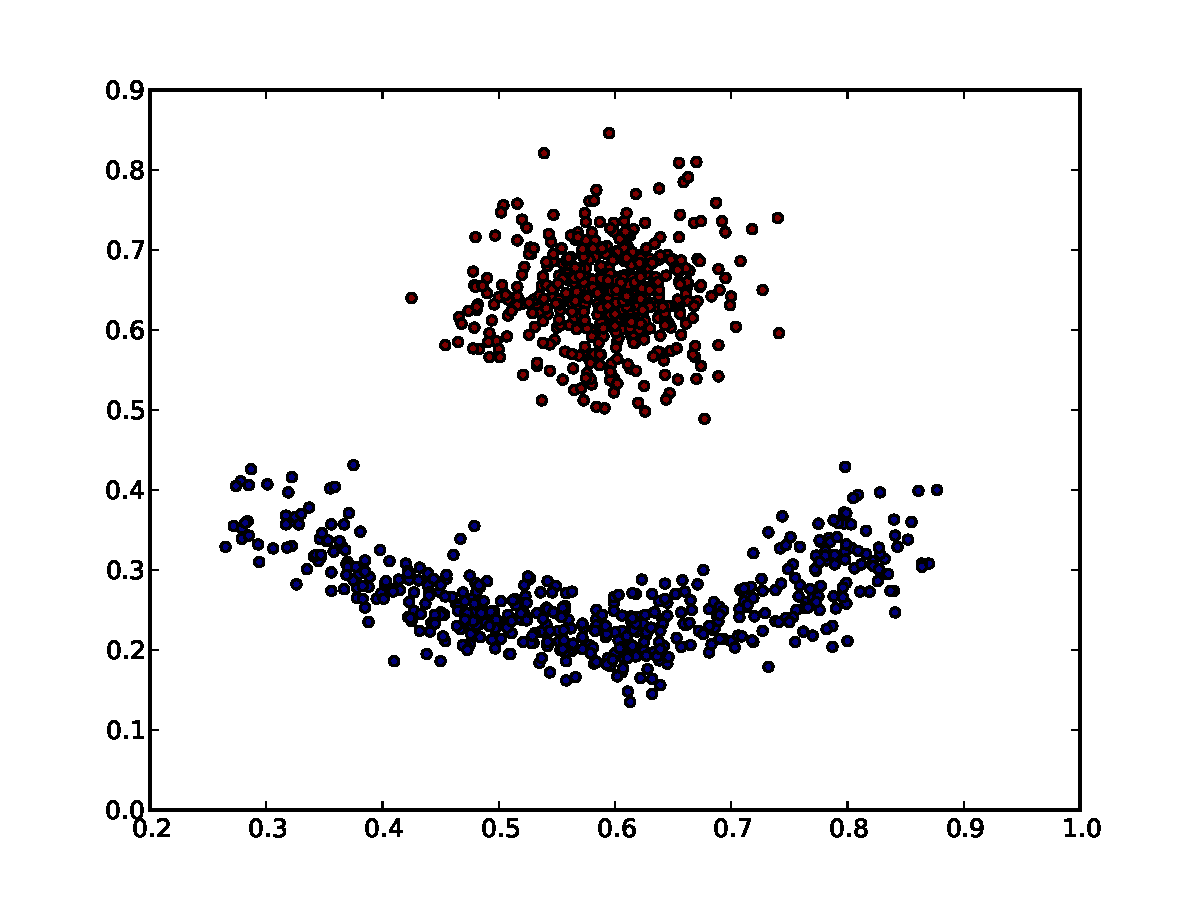
\includegraphics[scale=0.2]{red-blue-clusters.pdf}
            %\end{figure}
    %\end{itemize}
%\end{frame}

%\begin{frame}
%\frametitle{Podatki}
    %\begin{itemize}
       %\item Half-Moons
            %\begin{figure}[]
                %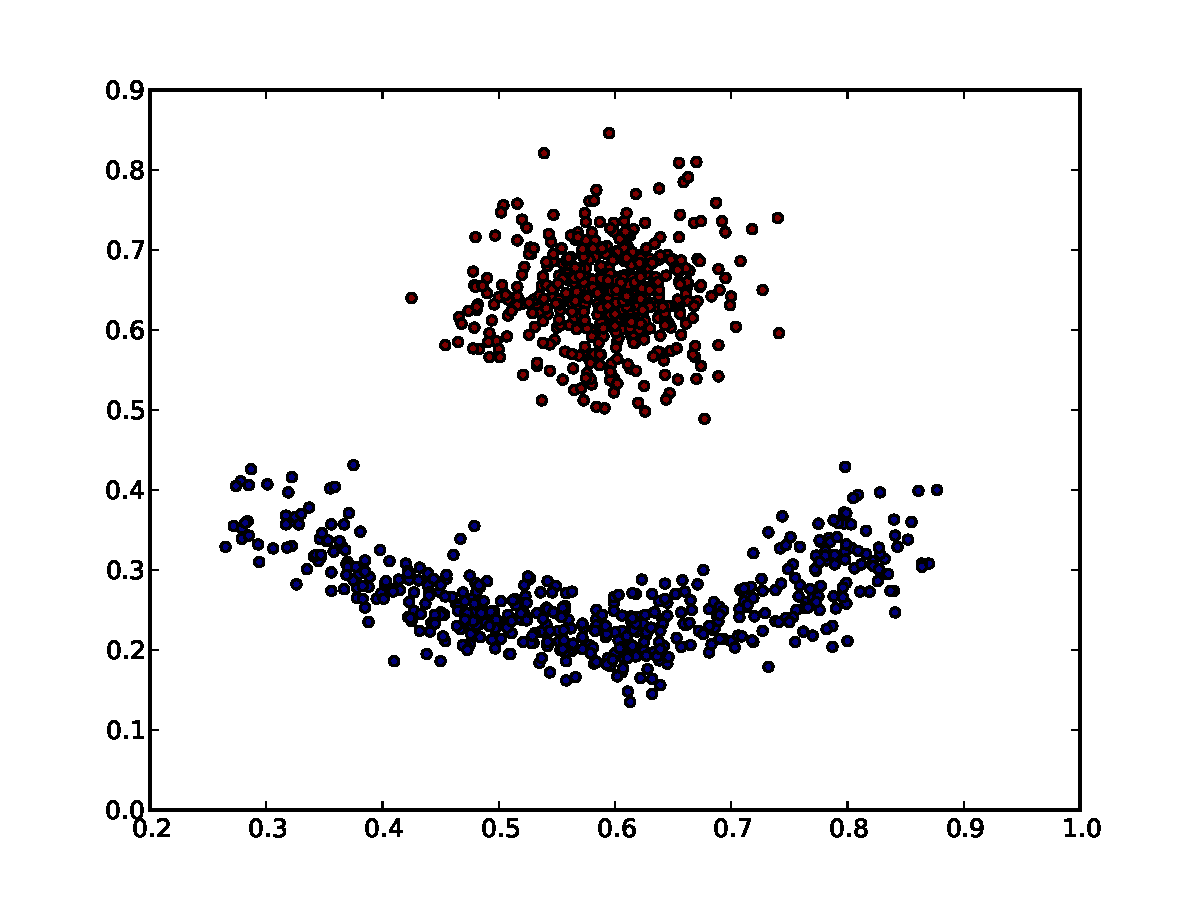
\includegraphics[scale=0.2]{red-blue-clusters.pdf}
            %\end{figure}
    %\end{itemize}
%\end{frame}

%\begin{frame}
%\frametitle{Algorithms}
    %\begin{itemize}
       %\item k-means
        %\item ECMC - Evolving Clustering Method with Constrained minimization
       %\item EM GMM - Expectation Maximization Gaussian Mixture Model
       %\item Spectral clustering
       %\item DBSCAN - Density-Based Spatial Clustering of Applications with Noise
    %\end{itemize}
%\end{frame}



%\begin{frame}
%\frametitle{k-means}
    %\begin{itemize}
       %\item Can produce undesirable results
       %\item Mostly very fast - k-means++
	%\item Used with other algorithms
    %\end{itemize}
%\end{frame}

\begin{frame}
\frametitle{k-means}
    \begin{figure}[]
    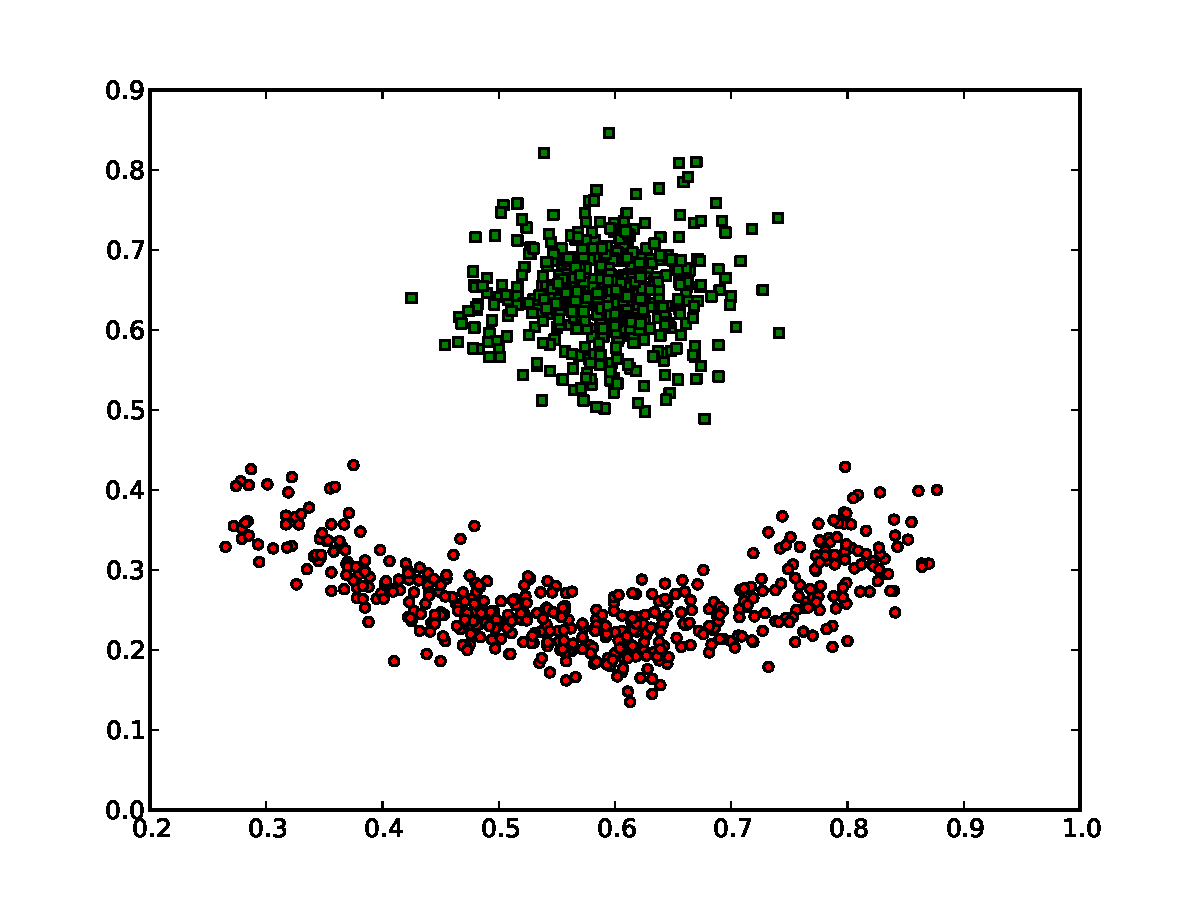
\includegraphics[scale=0.5]{kmeans_red-blue-clusters.pdf}
    \end{figure}
\end{frame}

\begin{frame}
\frametitle{k-means}
    \begin{figure}[]
    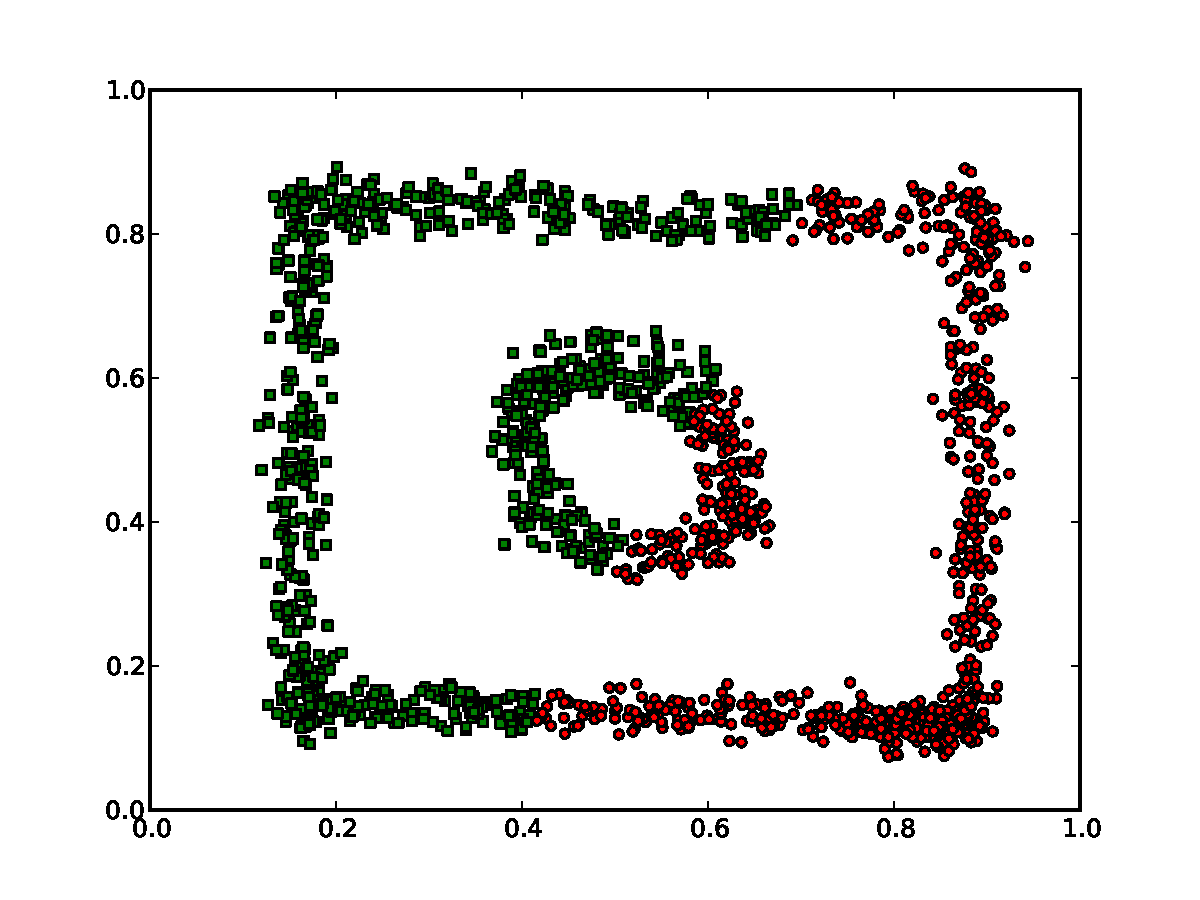
\includegraphics[scale=0.5]{kmeans_circle-weird.pdf}
    \end{figure}
\end{frame}

\begin{frame}
\frametitle{k-means}
    \begin{figure}[]
    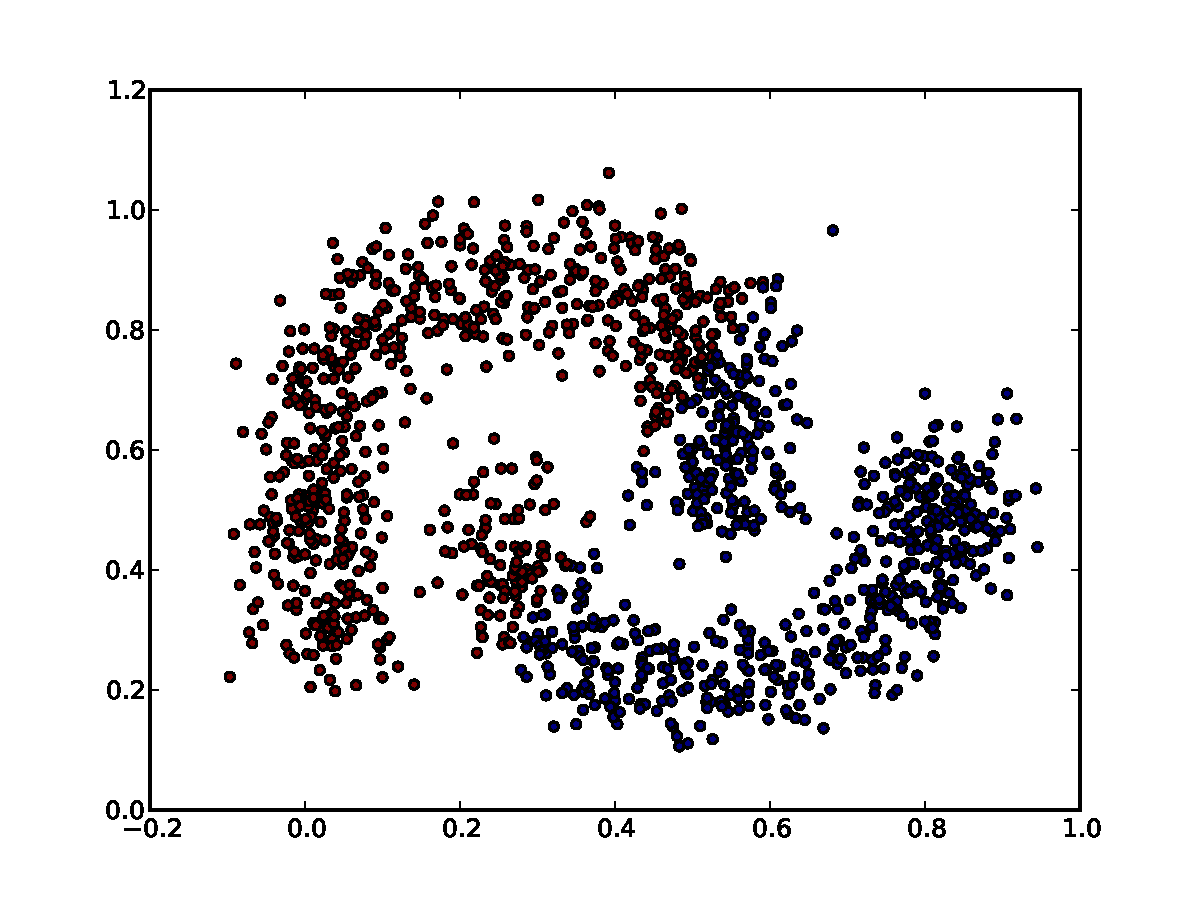
\includegraphics[scale=0.5]{kmeans_half-moons.pdf}
    \end{figure}
\end{frame}



\begin{frame}
\frametitle{ECMC}
    \begin{itemize}
	\item Distance based clustering
    	\item Constrained minimization
    \end{itemize}
\end{frame}

\begin{frame}
\frametitle{ECMC}
    \begin{figure}[]
    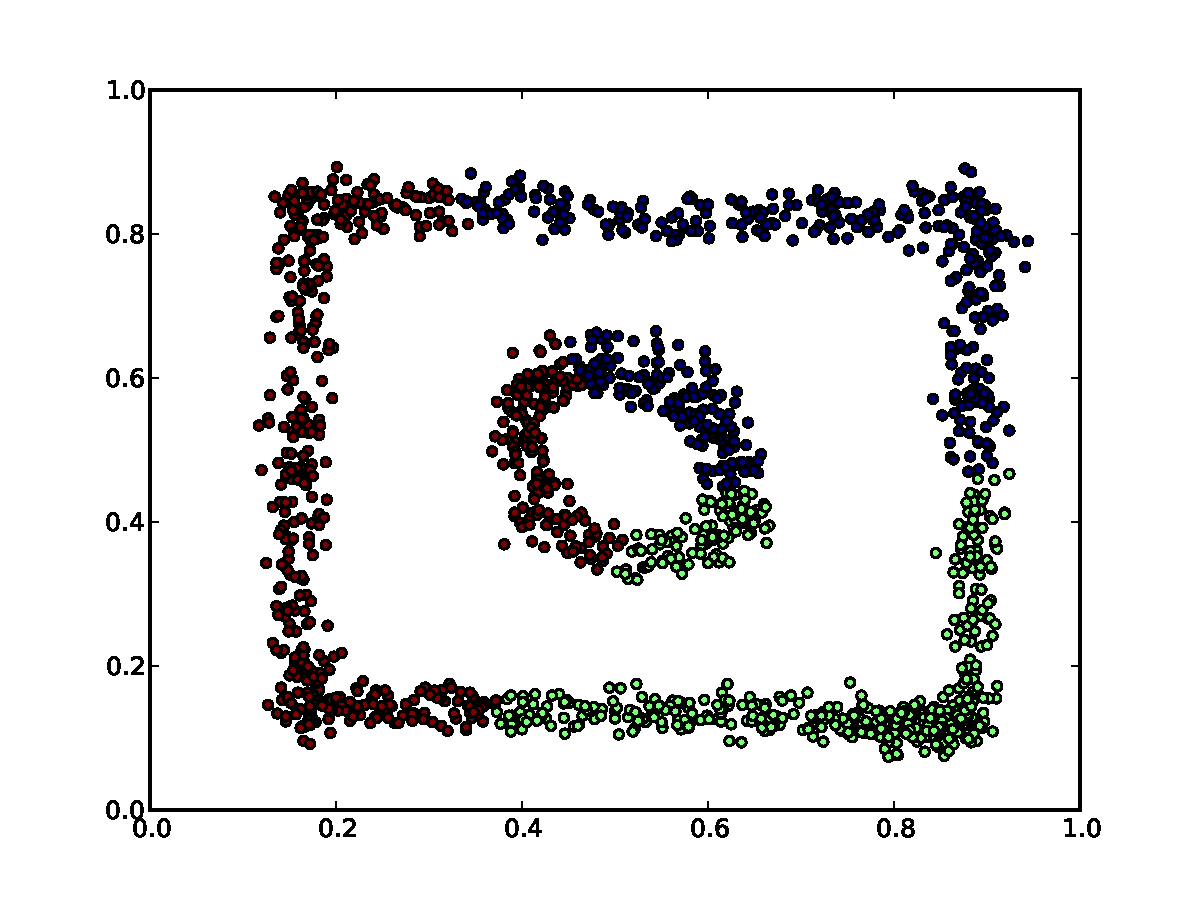
\includegraphics[scale=0.5]{ECMC_circle-weird.pdf}
    \end{figure}
\end{frame}

\begin{frame}
\frametitle{ECMC}
    \begin{figure}[]
    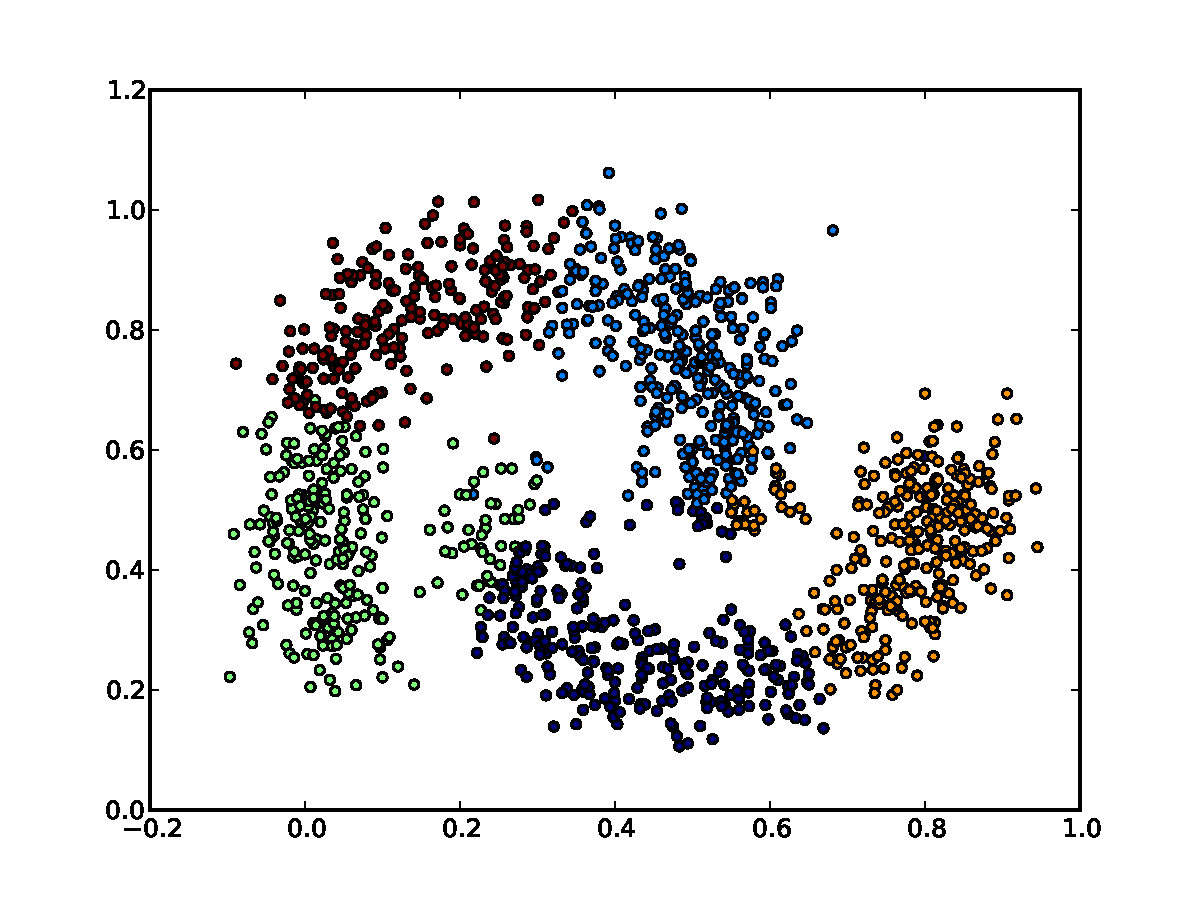
\includegraphics[scale=0.5]{ECMC_half-moons.pdf}
    \end{figure}
\end{frame}



\begin{frame}
\frametitle{EM GMM}
    \begin{itemize}
    	\item Statistical method
   	\item Mixture of Gaussian distributions
   	\item Using Expectation Maximization to find the solution
    \end{itemize}
\end{frame}

\begin{frame}
\frametitle{EM GMM}
    \begin{figure}[]
    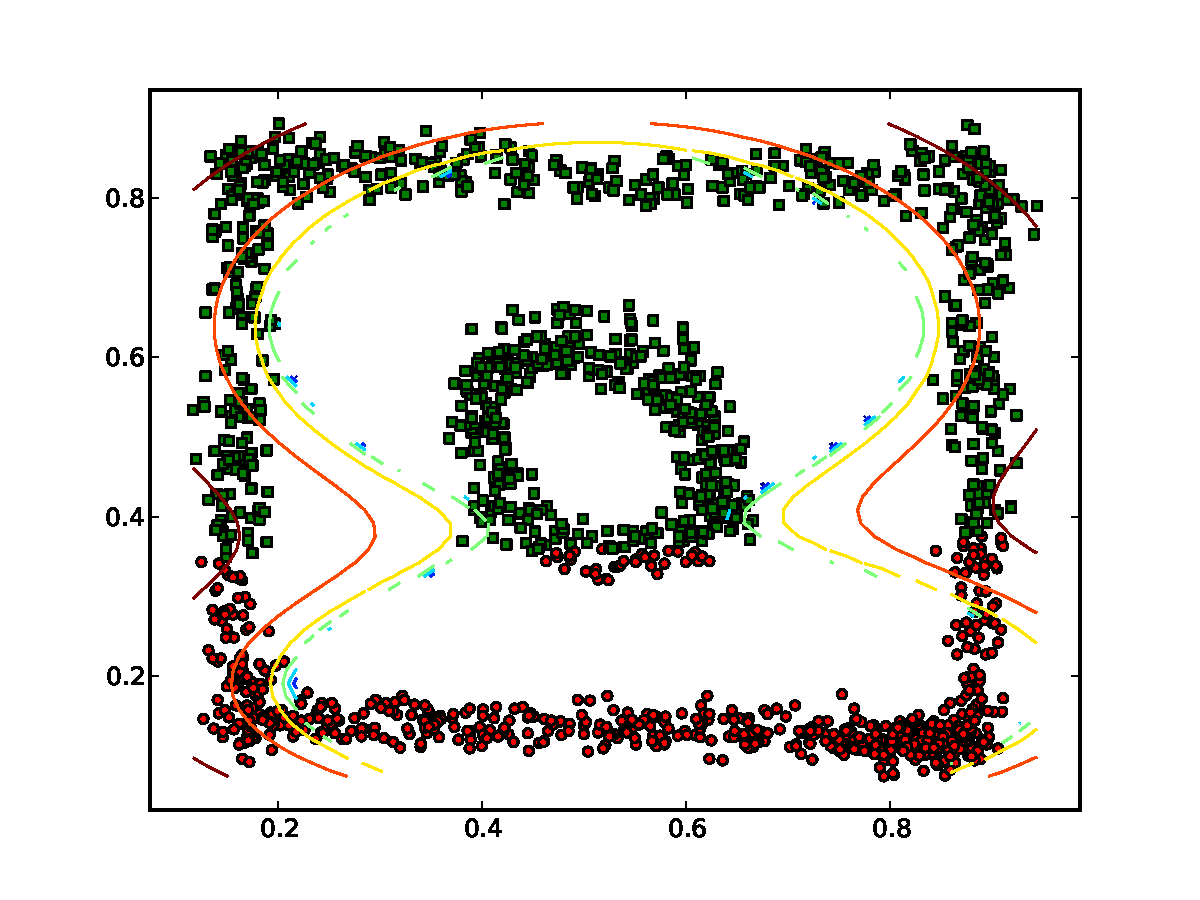
\includegraphics[scale=0.5]{GMM_circle-weird.pdf}
    \end{figure}
\end{frame}

\begin{frame}
\frametitle{EM GMM}
    \begin{figure}[]
    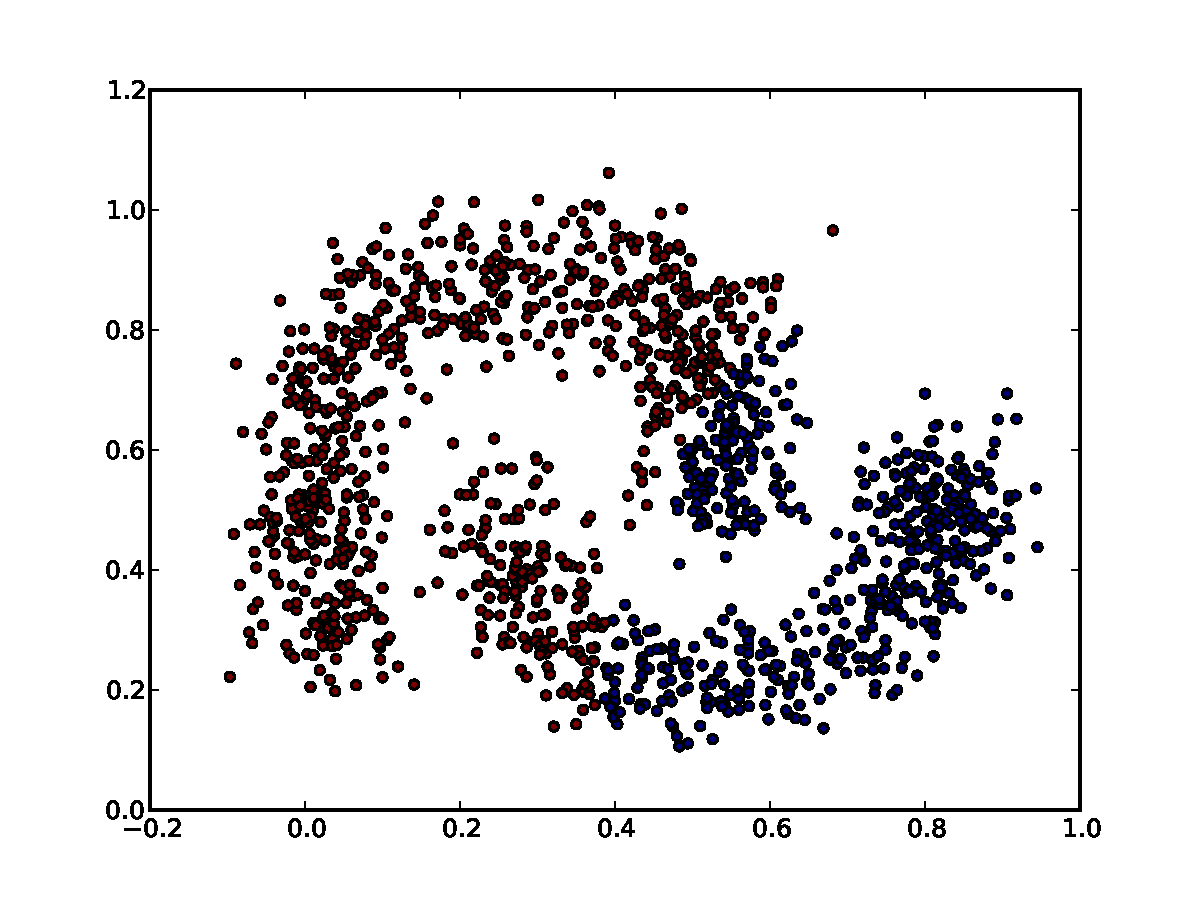
\includegraphics[scale=0.5]{GMM_half-moons.pdf}
    \end{figure}
\end{frame}



\begin{frame}
\frametitle{Spectral clustering}
    \begin{itemize}
	\item Graph-theoretic clustering
    	\item Uses standard linear algebra methods to perform dimensionality reduction
   	\item Similarity graphs and Laplacian matrices
    \item High computational complexity
    \end{itemize}

    \begin{center}
    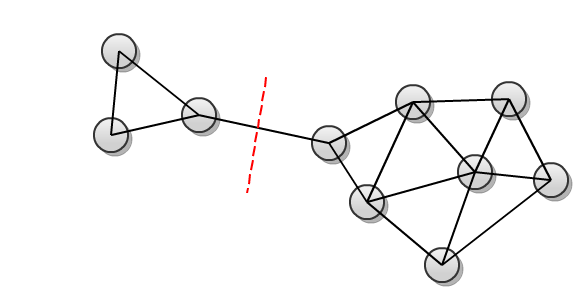
\includegraphics[scale=0.3]{spectral.png}
    \end{center}
\end{frame}

\begin{frame}
\frametitle{Spectral clustering}
    \begin{figure}[]
    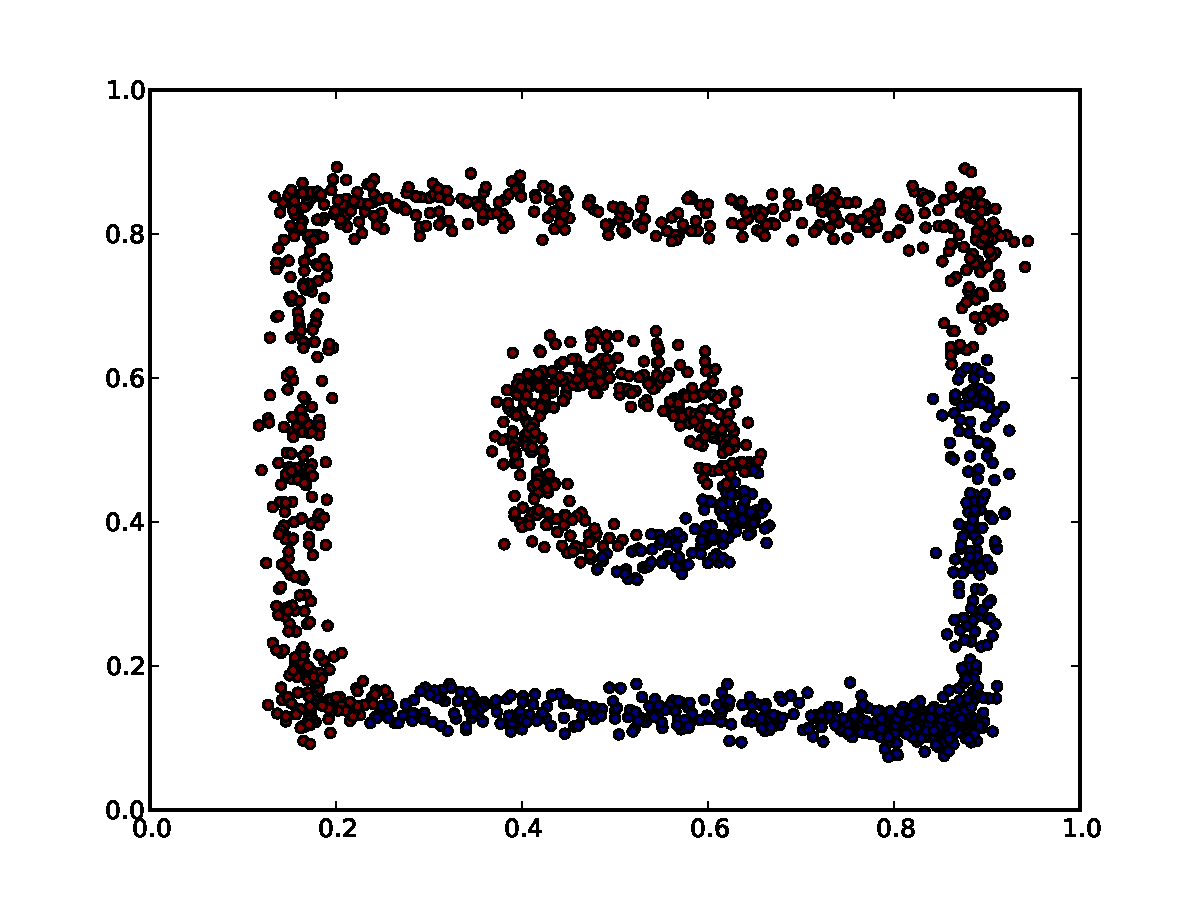
\includegraphics[scale=0.5]{spectral_circle-weird.pdf}
    \end{figure}
\end{frame}

\begin{frame}
\frametitle{Spectral clustering}
    \begin{figure}[]
    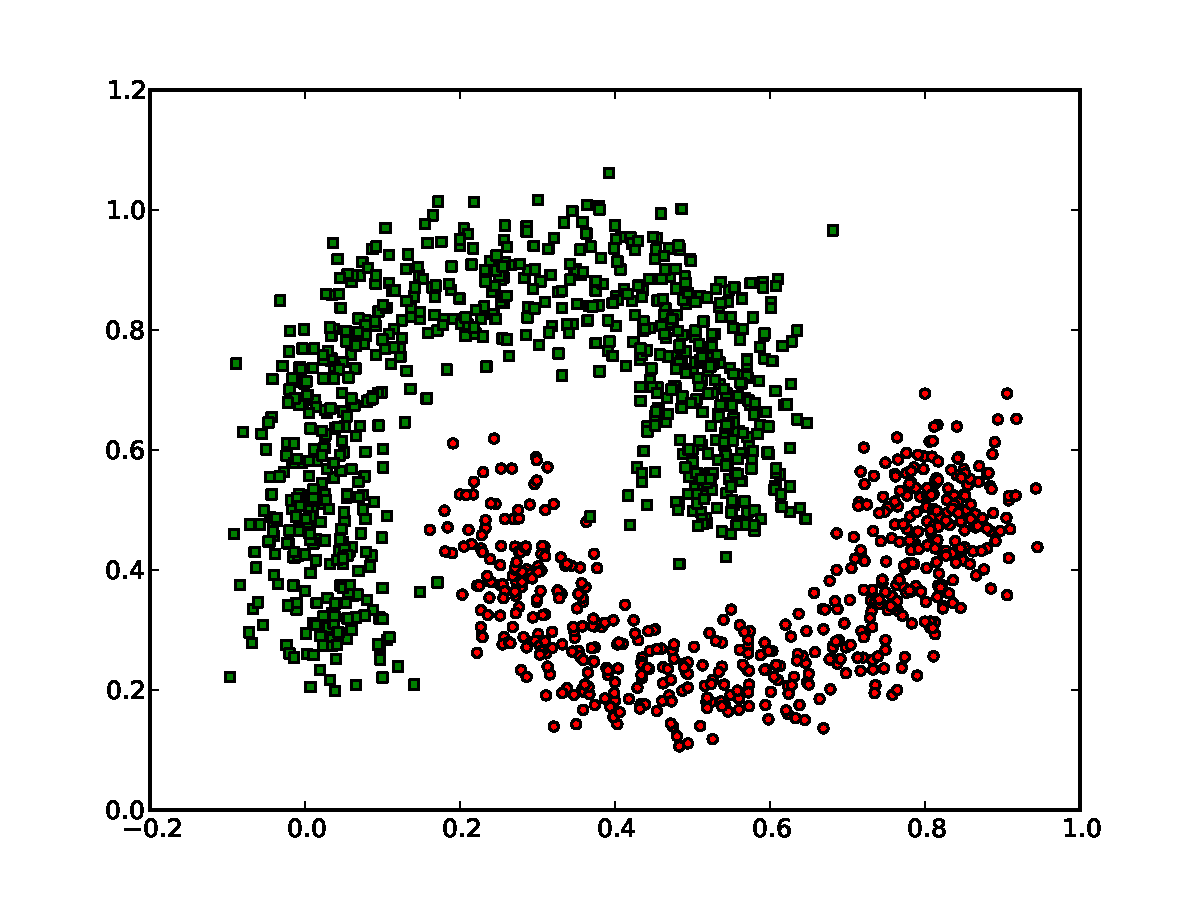
\includegraphics[scale=0.5]{spectral_half-moons.pdf}
    \end{figure}
\end{frame}



\begin{frame}
\frametitle{Density-based clustering}
    \begin{itemize}
    \item Clusters are areas of higher density
    \item No need to specify the number of clusters ($k$)
	\item DBSCAN best known, SNN, OPTICS...
    \item Noise detection
   	\item Fails on datasets with large differences in densities
    \end{itemize}
\end{frame}

\begin{frame}
\frametitle{Density-based clustering}
    \begin{figure}[]
    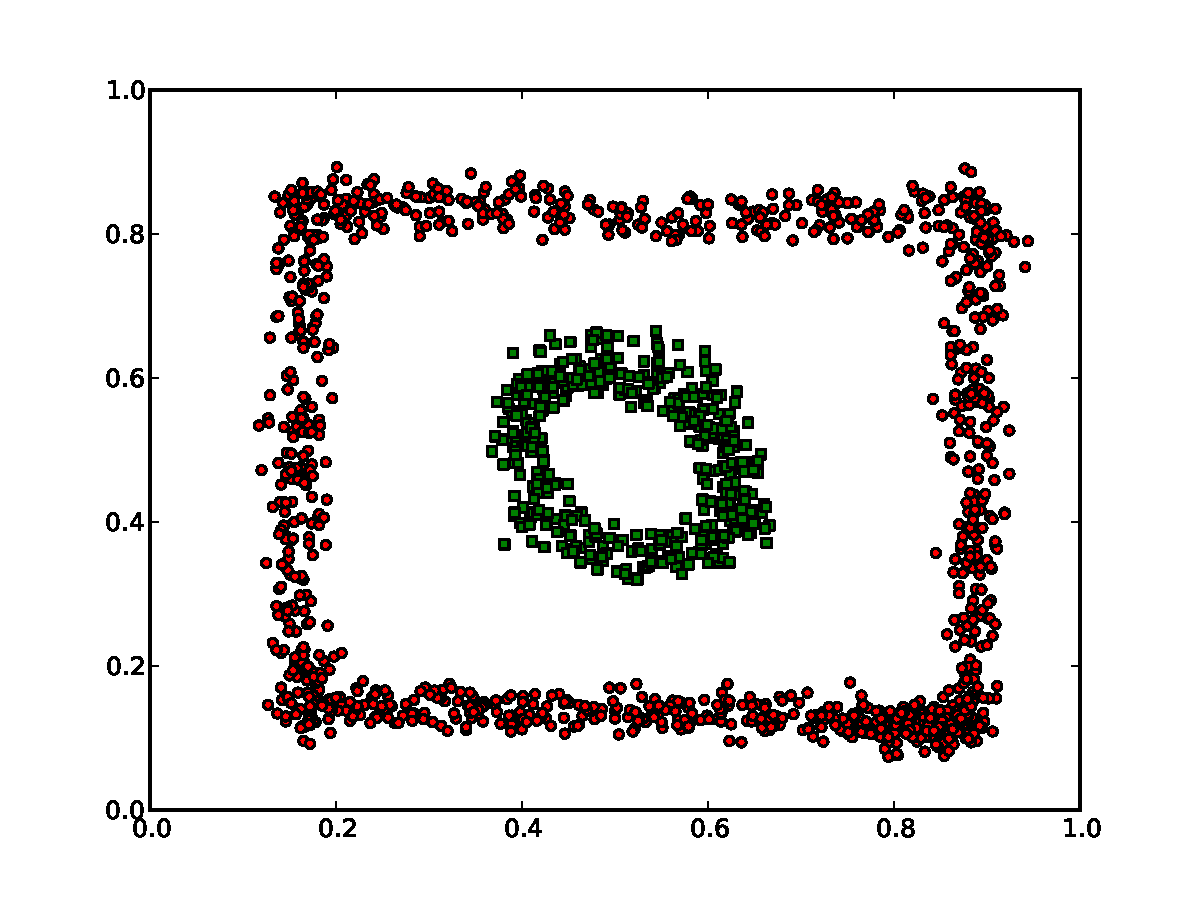
\includegraphics[scale=0.5]{dbscan_circle-weird.pdf}
    \end{figure}
\end{frame}

\begin{frame}
\frametitle{Density-based clustering}
    \begin{figure}[]
    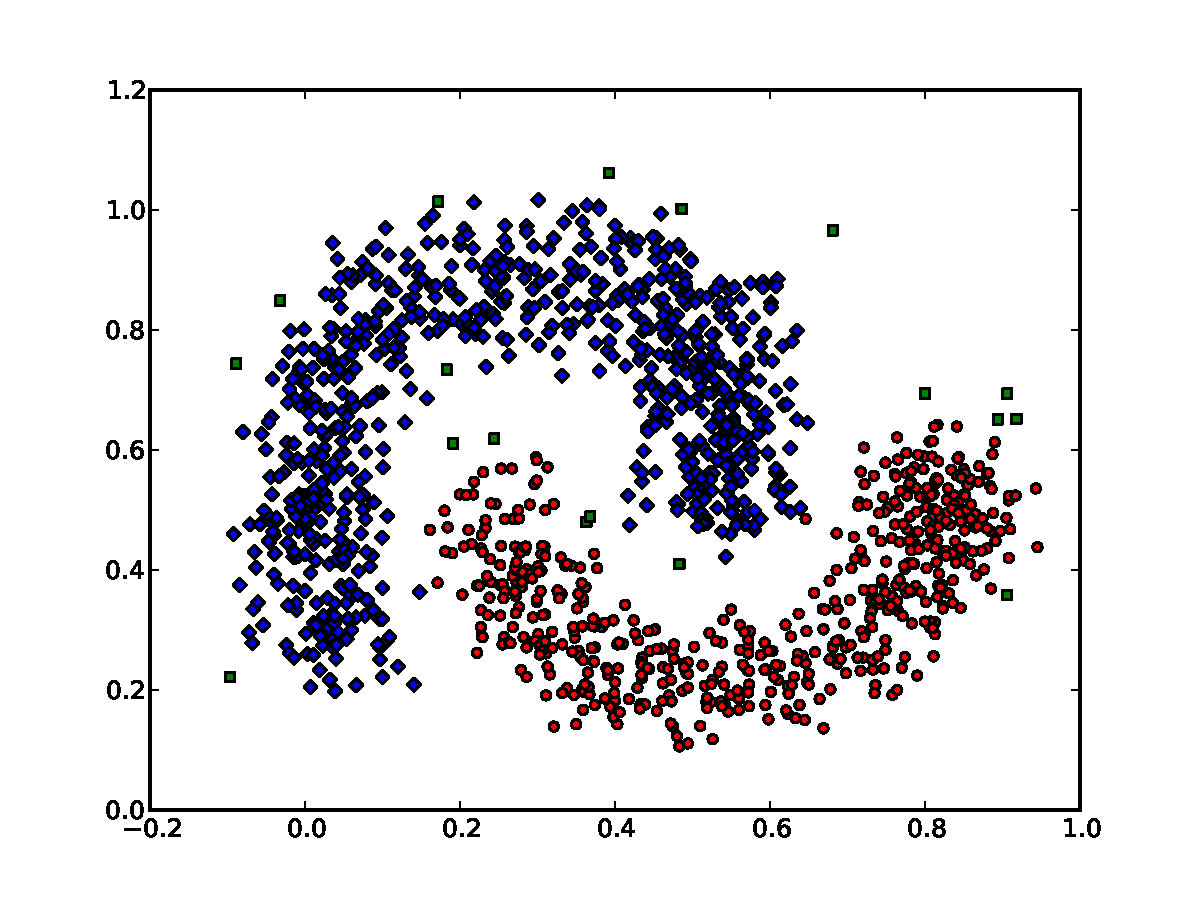
\includegraphics[scale=0.5]{dbscan_half-moons.pdf}
    \end{figure}
\end{frame}


\begin{frame}
\frametitle{Conclusions}
    \begin{itemize}
	\item Spectral clustering best overall in our tests
    	\item DBSCAN close second (noise detection)
	\item Other algorithms had problem with complex problems

   	\item Appropriate algorithm must be chosen for problem
    \end{itemize}
\end{frame}


\end{document}
